\section{Recorded Data Products and Positioning Capabilities}
\label{sec:capabilities}

ARFT exposes several distinct data products, each corresponding to a different layer of the workflow. At acquisition time, the rover logger writes one CSV row per completed move, the \gls{rf} clients write one runtime record per hostname and cycle, and the \gls{rf} orchestrator writes one YAML summary entry per synchronized cycle. The post-processing path then converts these operational files into analysis-ready NetCDF products. The use of hierarchical NetCDF products for the released tensors is also consistent with broader 6G testbed efforts that standardize reusable measurement datasets on top of NetCDF/HDF5 storage backends~\cite{dss6g}.

The current merged \gls{rf} NetCDF aggregates EXP003 and EXP005--EXP012 and has dimensions \texttt{experiment\_id} $\times$ \texttt{cycle\_id} $\times$ \texttt{hostname}. Its main variables are \texttt{csi\_real}, \texttt{csi\_imag}, \texttt{csi\_available}, \texttt{rover\_x}, \texttt{rover\_y}, \texttt{rover\_z}, and \texttt{position\_available}. One physical \gls{rf} observation is reconstructed as \texttt{csi\_real} $+ j\,\texttt{csi\_imag}$, while \texttt{csi\_available} indicates whether a given \texttt{(experiment\_id, cycle\_id, hostname)} tuple is populated. This design gives the user both direct array access and an explicit validity mask.

The \gls{rf} product should be interpreted as a distributed spatial fingerprint of the rover location. Each cycle yields a 42-element complex vector over the ceiling tiles, derived from the per-host pilot phase and amplitude measurements after cable correction. Across the 5011 populated \gls{rf} cycles in the merged file, the dataset stores 210068 tile-level complex \gls{csi} samples. Host coverage is also strong: 4617 of the 5011 \gls{rf} cycles contain all 42 ceiling-tile entries, and the remaining 394 cycles contain 41 entries. In other words, the typical measurement point is not a sparse partial vector but a nearly complete 42-element spatial snapshot. This makes the \gls{rf} modality directly usable for fingerprint-based positioning, for geometry-aware inference that exploits the distributed aperture, and for learning spatial channel maps that are later inverted for localization.

The acoustic product complements this with waveform-level information. The acoustic pipeline writes one NetCDF per experiment with waveform data organized on \texttt{(experiment\_id, cycle\_id, microphone\_label, sample\_index)}. Each stored trace corresponds to the chirp response recorded by a microphone at the same rover stop as the paired \gls{rf} snapshot. The acoustic modality therefore preserves time-domain propagation structure such as direct-path timing, reverberation, and multipath signatures. These traces can be used for acoustic fingerprinting, feature extraction for position regression or classification, or model-based processing that uses arrival-time and room-response cues for localization.

The key capability is tri-modal alignment. Because the acoustic and \gls{rf} parsers use the same \texttt{(experiment\_id, cycle\_id)} key, ARFT supports direct cycle-level joining between rover position, tile-level \gls{rf} channel measurements, and raw microphone waveforms. Since each cycle also has a ground-truth rover pose from Qualisys, the release supports three natural positioning regimes: RF-only positioning, acoustic-only positioning, and joint multimodal positioning in which both feature sets are fused against the same $(x,y,z)$ target. \Cref{fig:rf-acoustic-position-waveforms,fig:csi-position-heatmaps} show two notebook-derived views of this alignment and \gls{rf} structure: one cycle-level acoustic waveform matrix joined to a selected \gls{rf} position, and phase/amplitude heatmaps over a sequence of \gls{rf} cycles.

\begin{figure}[t]
    \centering
    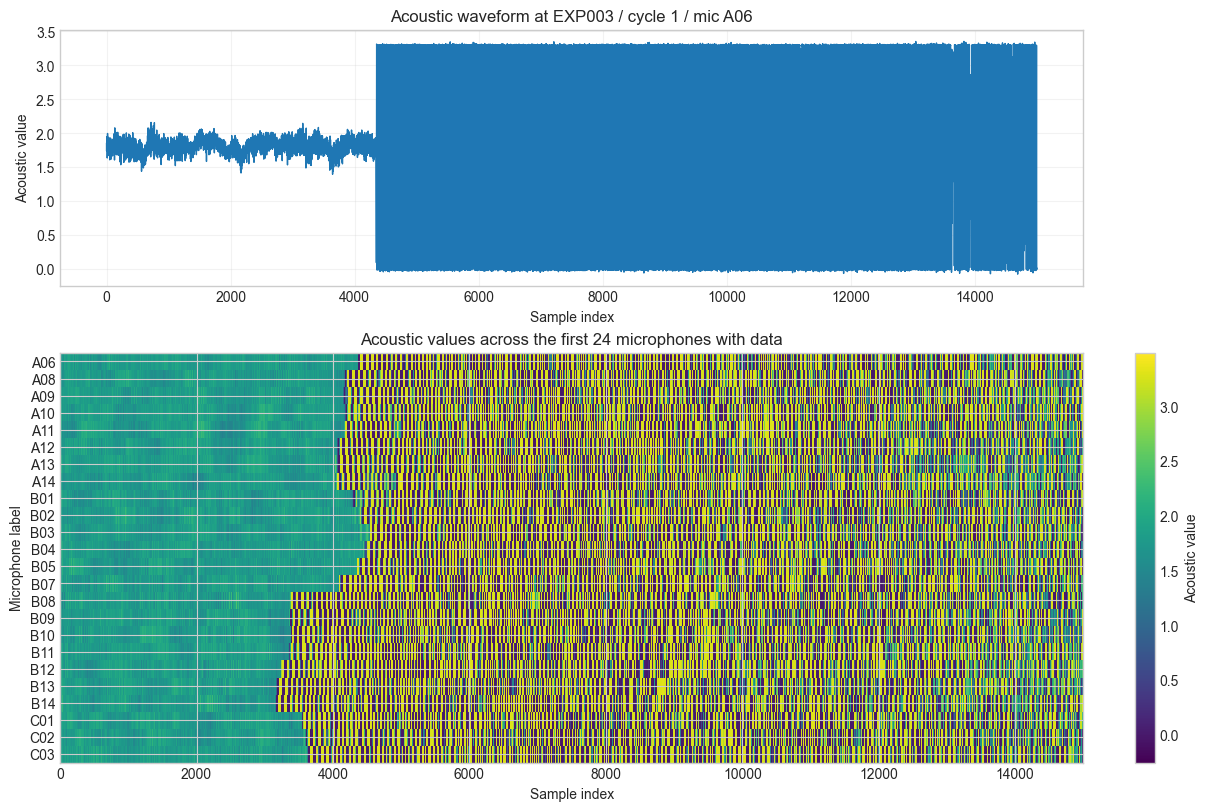
\includegraphics[width=0.5\textwidth]{figures/notebook-exports/rf_acoustic_position_waveform_heatmap.png}
    \caption{Acoustic waveform inspection for the position resolved by the joint \gls{rf}-acoustic notebook. The upper panel shows one microphone trace for \texttt{EXP003}/cycle~1, while the lower panel shows the corresponding waveform matrix for the first microphones with available data at the same acquisition cycle.}
    \label{fig:rf-acoustic-position-waveforms}
\end{figure}

\begin{figure}[t]
    \centering
    \begin{subfigure}[t]{0.48\textwidth}
        \centering
        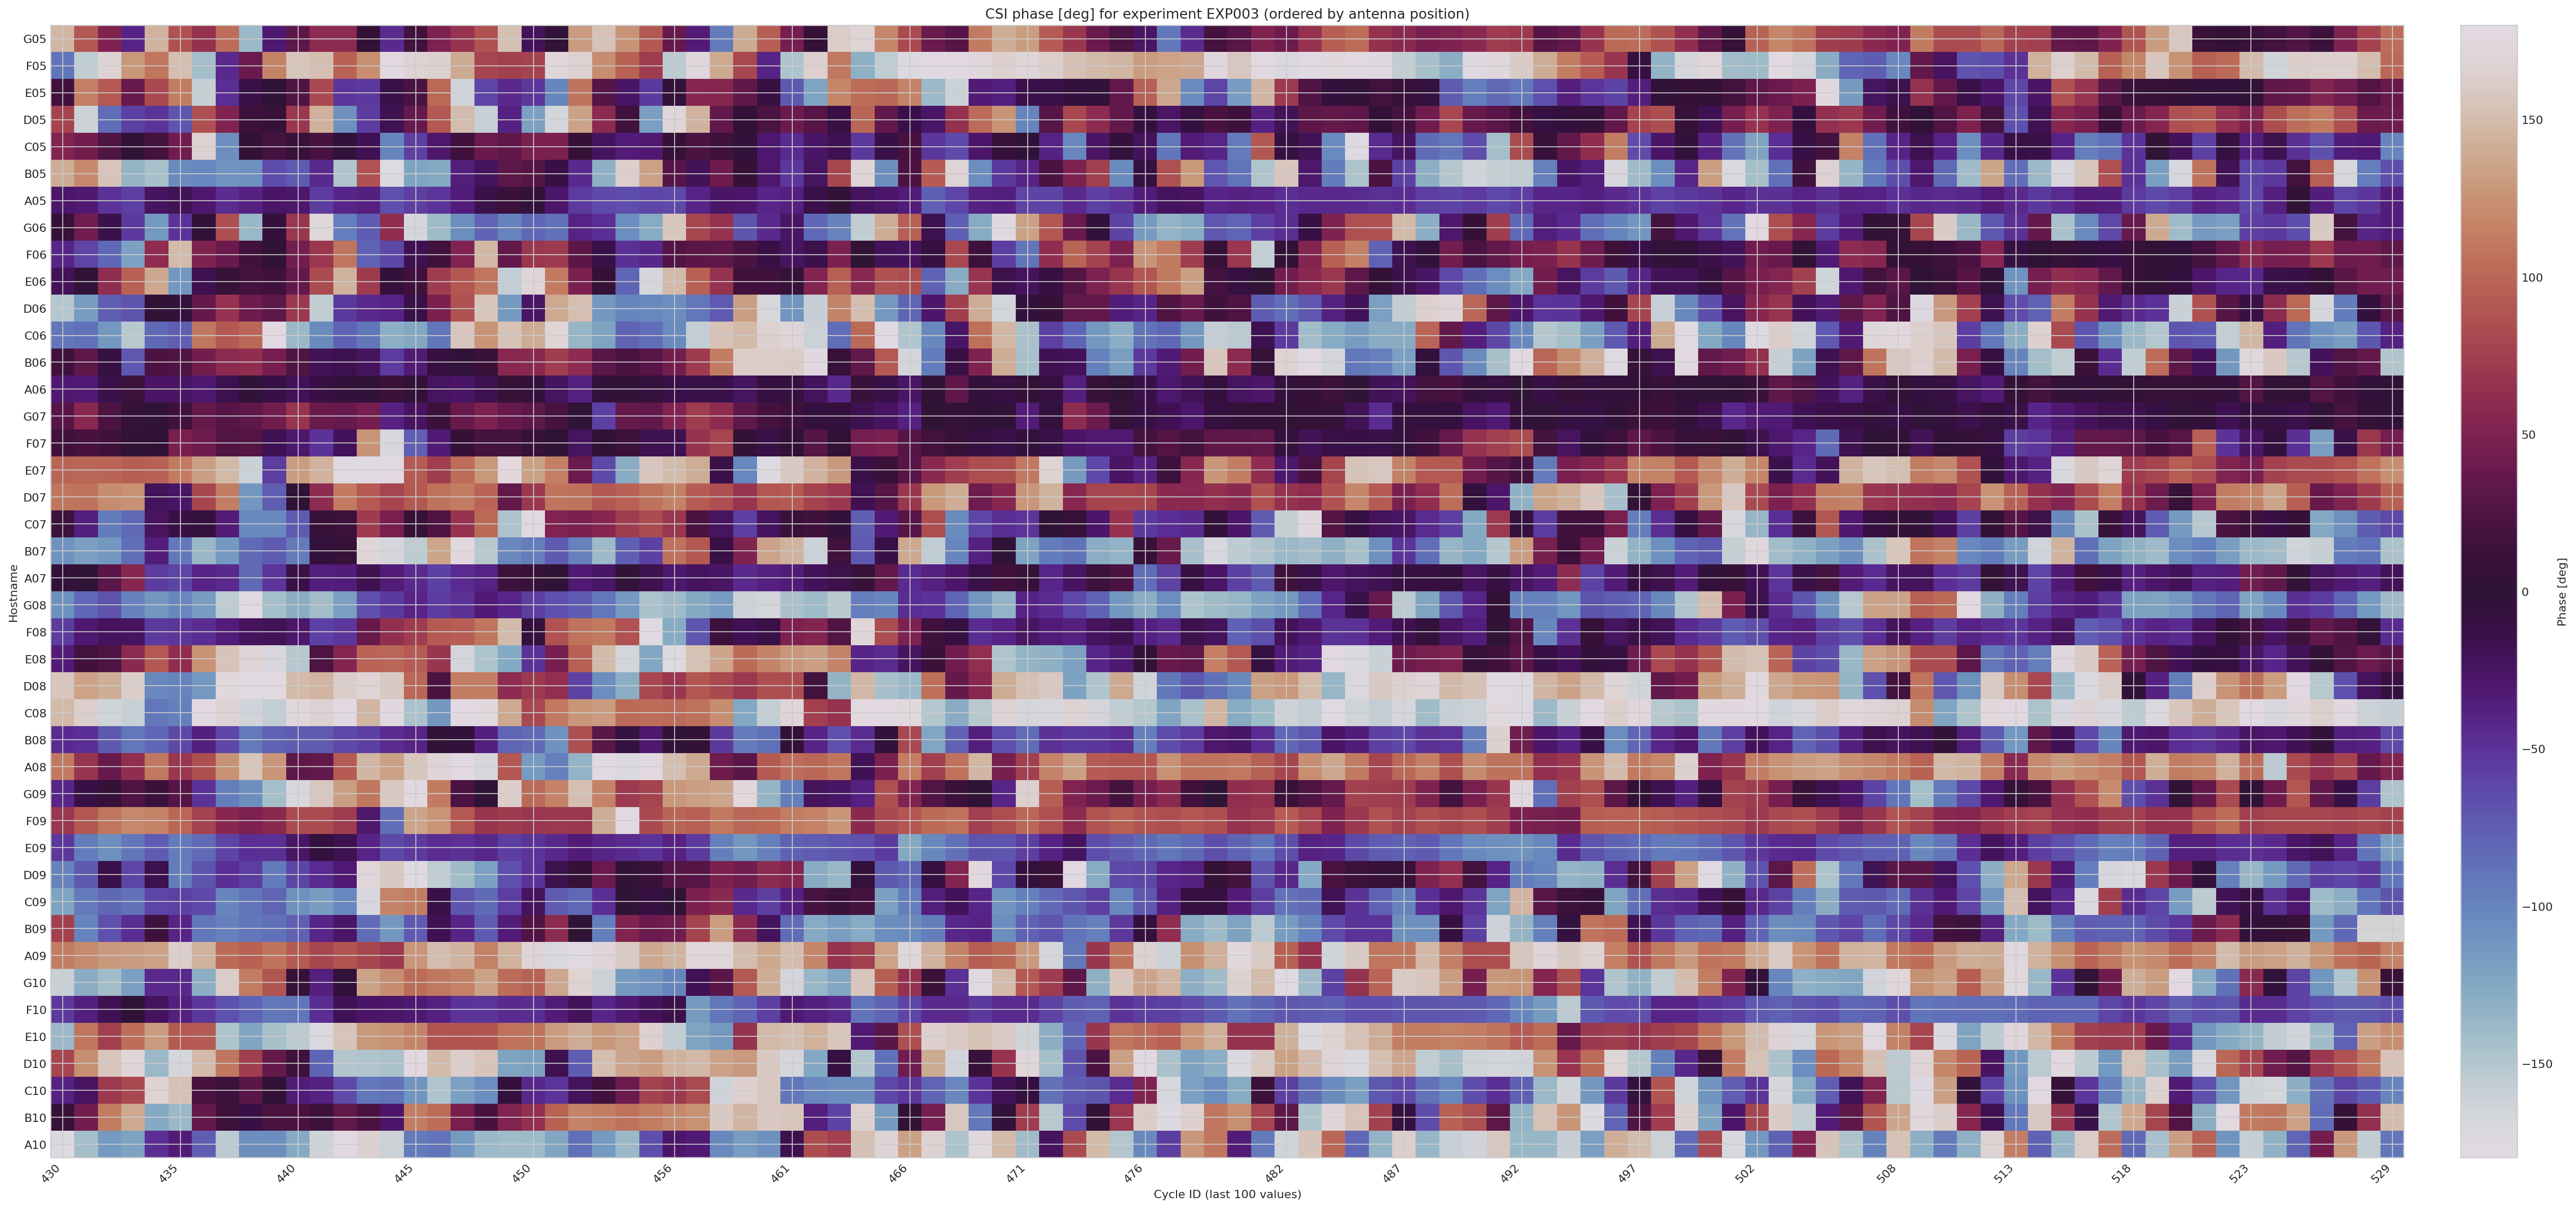
\includegraphics[width=\linewidth]{figures/notebook-exports/csi_position_phase_heatmap.png}
        \caption{\gls{csi} phase over the selected cycle window.}
    \end{subfigure}\hfill%
    \begin{subfigure}[t]{0.48\textwidth}
        \centering
        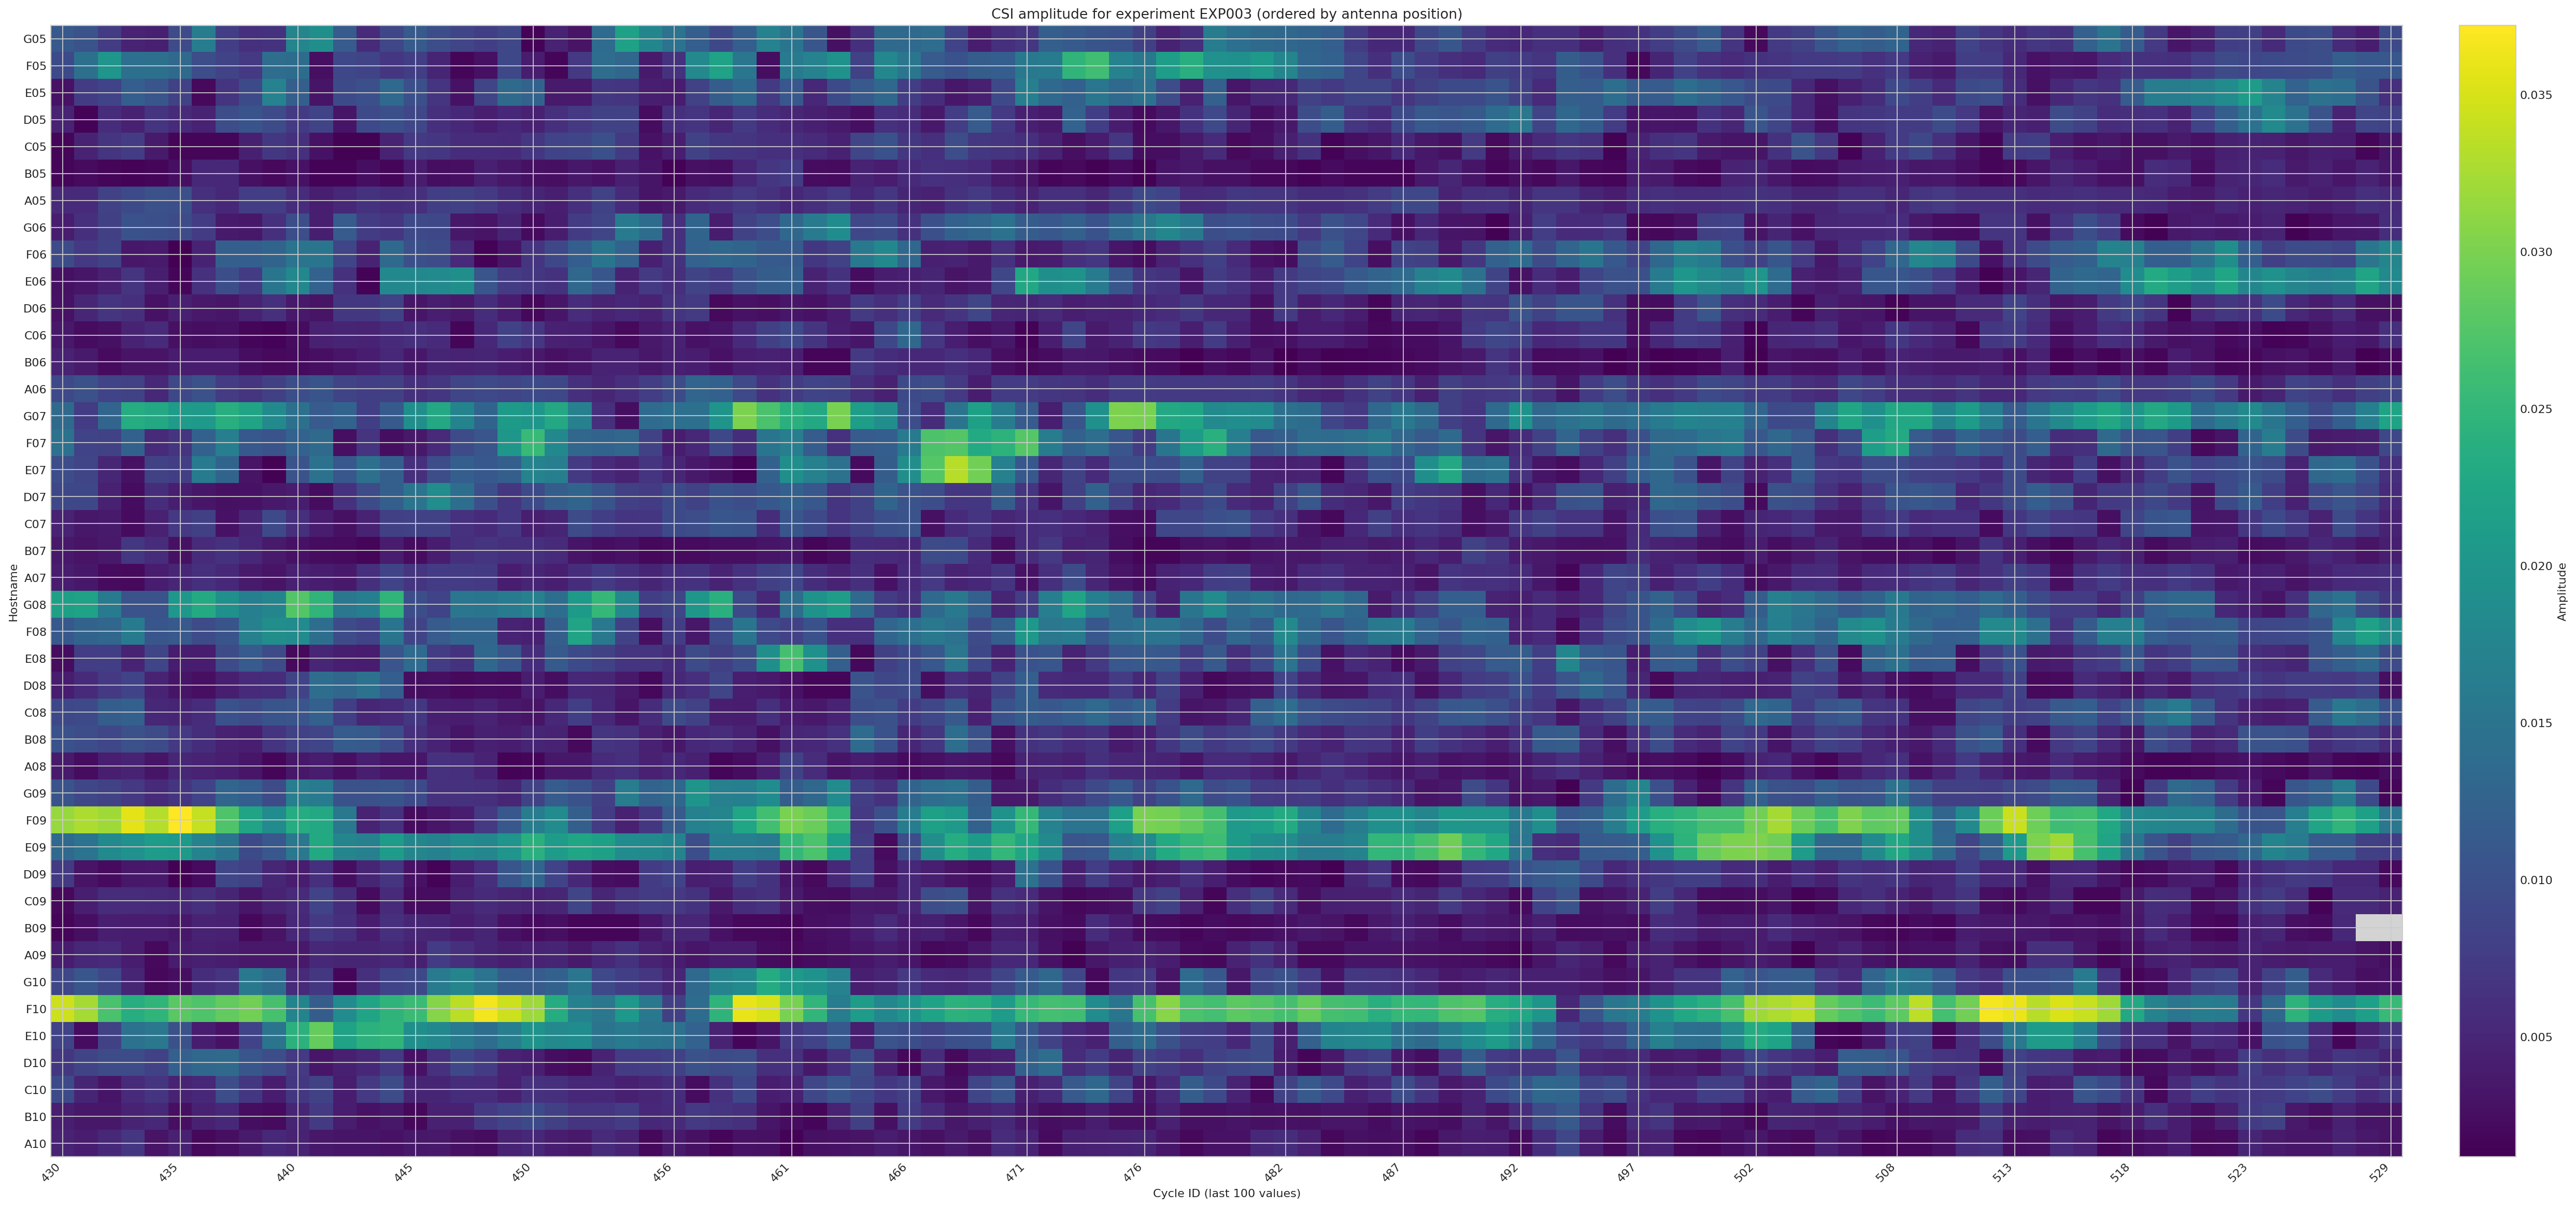
\includegraphics[width=\linewidth]{figures/notebook-exports/csi_position_amplitude_heatmap.png}
        \caption{\gls{csi} amplitude over the same cycle window.}
    \end{subfigure}
    \caption{Heatmaps from \texttt{tutorial\_csi\_per\_position.ipynb}. The rows are ordered ceiling receiver hostnames, and the columns show the final cycle IDs in the selected experiment window. Together they expose stable receiver-dependent structure and temporal variation in the \gls{rf} channel tensor.}
    \label{fig:csi-position-heatmaps}
\end{figure}


\begin{figure*}[b]
    \centering
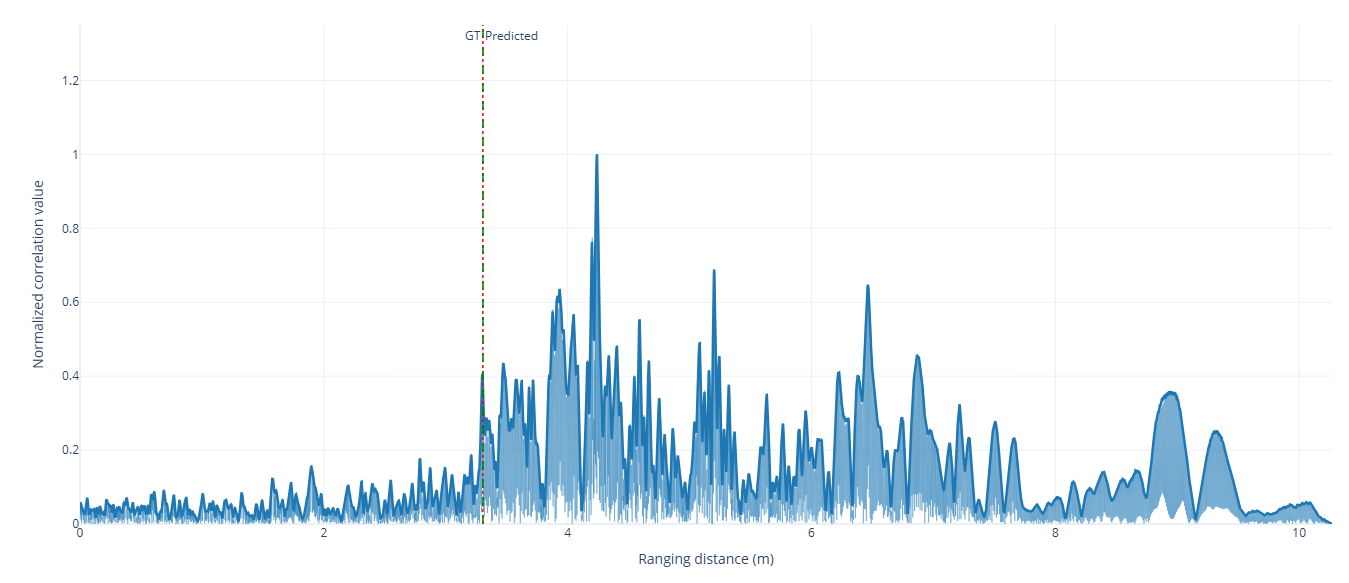
\includegraphics[width=0.9\textwidth]{article/figures/correlation_graph_good_example.png}
    \caption{Ranging estimate example for cycle 304 EXP007 microphone C04 with the correlation values and LPF values. The correct peak resulting in the estimated range is determined using the peak-prominence algorithm. The estimated and ground-truth range is depicted.}
    \label{fig:correlation_graph_example}
\end{figure*}

\begin{figure}[]
    \centering
    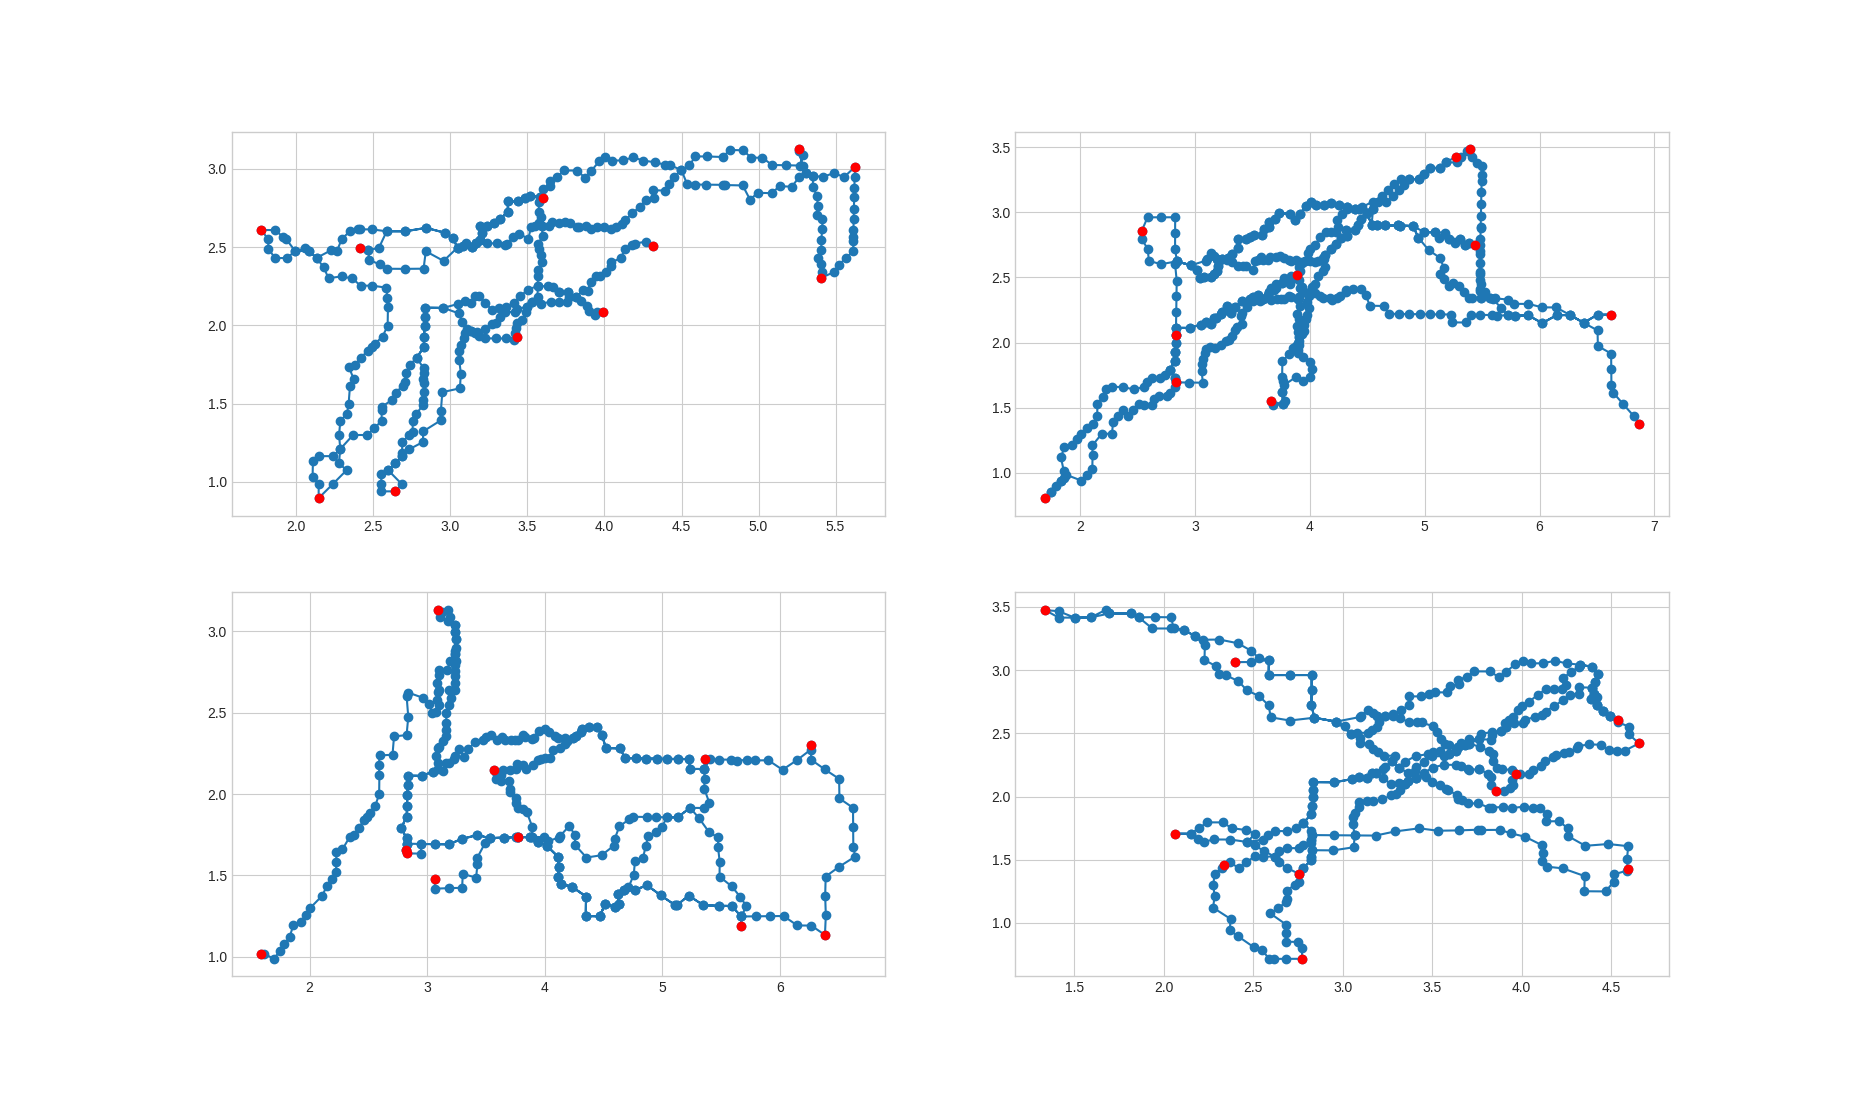
\includegraphics[width=\linewidth]{article/figures/paths.png}
    \caption{Four randomly generated walks. Red indicates a static point, and blue indicates points on the paths between static points.}
    \label{fig:generatedwalks}
\end{figure}

The post-processing workspace now makes the RF--acoustic positioning path concrete rather than merely hypothetical. It includes a graph-based walk generator and persisted train/test trajectory splits, with 2500 generated training walks and 50 held-out test walks. The test set positions are excluded from the training walks data.
The walk generator works by choosing a sequence of static flagged positions, and repeatedly performing Dijkstra's algorithm to find the shortest path from one static point to the next, along the rover measurement points. Static positions are introduced to perform acoustic positioning. The sequence of static points can either be randomly generated or manually specified. There is also an option to forbid the paths from containing specific points. Figure \ref{fig:generatedwalks} showcases four examples of randomly generated walks.

The acoustic positioning scripts operate on the static flagged positions in the paths by filtering the received signals, selecting anchor microphones, applying chirp pulse compression as depicted in Fig.~\ref{fig:correlation_graph_example}, estimating time-of-arrival ranges based on a peak-prominence algorithm, and by determining a least-squares position estimate for each rover stop. The most optimal peak-prominence-factor is determined for this dataset, resulting in a value equal to 0.24.  The current configuration uses up to 50 selected anchors per stop with sum-rate-based ranking due to the saturating operation mode of the microphones, which means that the released waveform data is already exercised by a full end-to-end model-based localization pipeline. 

The saved evaluation artifacts are strong enough to summarize as experimental evidence. The calibrated acoustic results cover 50 held-out paths and 550 localized rover stops. Across that set, the mean 2D positioning error is 0.110~m and the P90 value is equal to 0.195~m, while the mean 3D positioning error is 0.130~m and the P90 value is equal to 0.217~m. The accompanying ranging records contain 27500 anchor-wise distance estimates with mean absolute error 0.311~m. These values should be interpreted as documented baseline performance of the current model-based acoustic pipeline, not as an upper bound on what the dataset can support. At present, the \gls{rf} pipeline regarding positioning is still exploratory compared with the more complete acoustic ranging-and-localization path. \Cref{fig:capability-artifacts} illustrates tile-level interpretation of one synchronized \gls{rf} capture. This is a meaningful capability distinction for users who may be interested in fingerprinting, distributed channel modeling, RF-acoustic fusion, or direct positioning inference.

\begin{figure}[t]
    \centering
    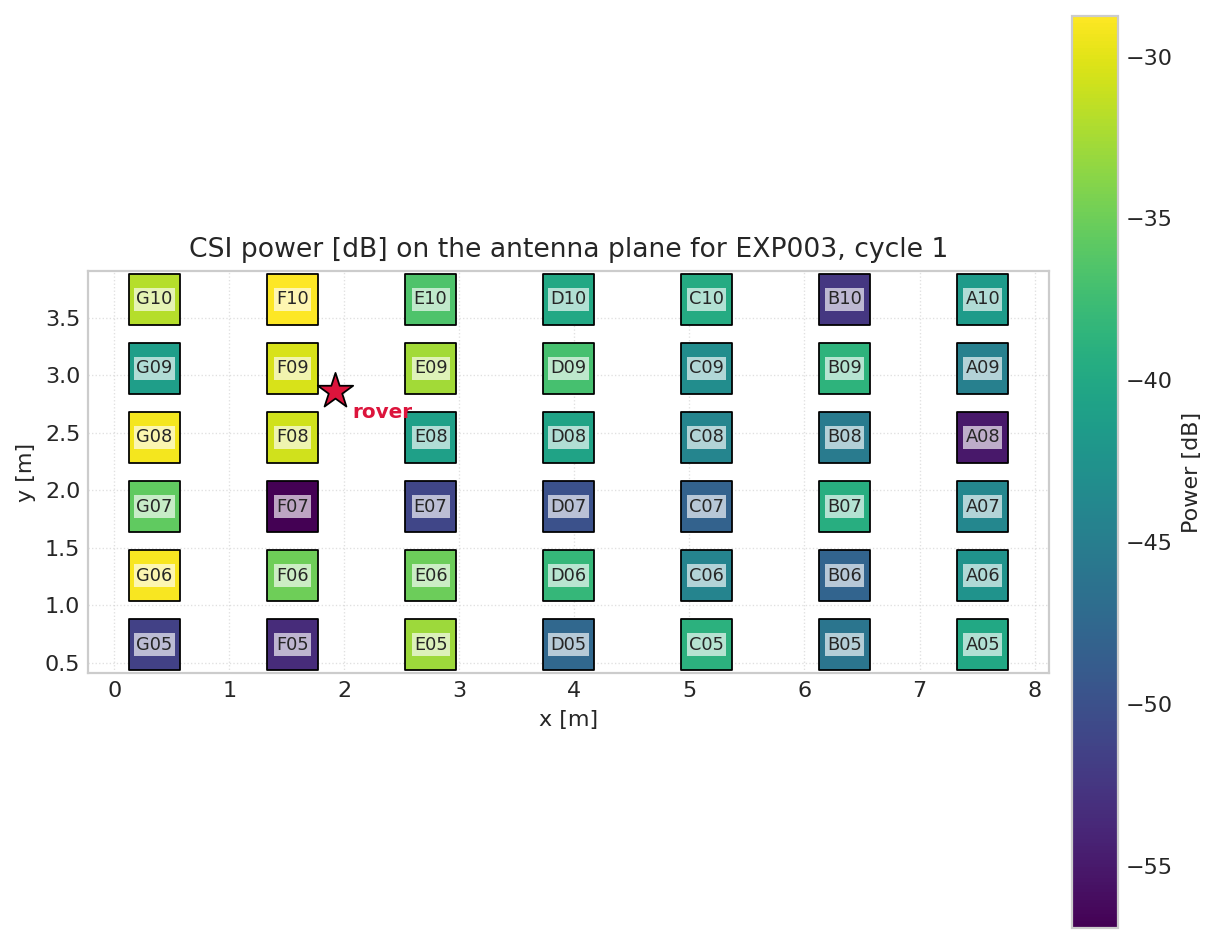
\includegraphics[width=\linewidth]{figures/notebook-exports/csi_spatial_power_snapshot.png}
    \caption{Example per-position \gls{rf} power snapshot over the 42 ceiling receivers.}\label{fig:capability-artifacts}
\end{figure}

The analysis workflow already demonstrates the most immediate downstream uses. The provided notebooks support:
\begin{itemize}
    \item campaign-level trajectory inspection and measurement-cloud visualization;
    \item overview heatmaps of \gls{csi} phase and amplitude over the measurement set;
    \item single-position spatial snapshots across the 42 ceiling receivers;
    \item joint \gls{rf}-acoustic inspection at a selected rover stop;
    \item export of movie sequences showing spatial evolution of phase and power.
\end{itemize}
Taken together with the acoustic and \gls{rf} post-processing scripts, these are not promised future tasks, they are concrete analyses already represented by scripts, notebooks, and exported figures in the present project release.




